\section{Szenariokonstruktion}
\label{constructions}
Als dritte und wichtigste Phase der Szenarioanalyse werden nun Szenarien aus den vorher definierten Einflussfaktoren erstellt. Hierfür bietet es sich an, die vorher ermittelten Entwicklunsausprägungen der einzelnen Schlüsselfaktoren auf Widerspruchsfreiheit zu überprüfen . Dafür wird eine Konsistenzanalyse genutzt \cite{spath}. Auf dessen Grundlage werden danach zukunftsfähige Anwendungsszenarien für die Skola GmbH erstellt.

\subsection{Konsistenzanalyse}

In der in Abbildung \ref{fig:konsistenzanalyse} dargestellten Konsistenzanalyse erhält man eine Übersicht über die Beziehung zwischen den einzelnen Ausprägungen. Der Übersichtlichkeit halber wurden die einzelnen Ausprägungen abgekürzt. Die Erklärungen finden sich in Abschnitt \ref{manifestations}.

\begin{figure}
	\centering
	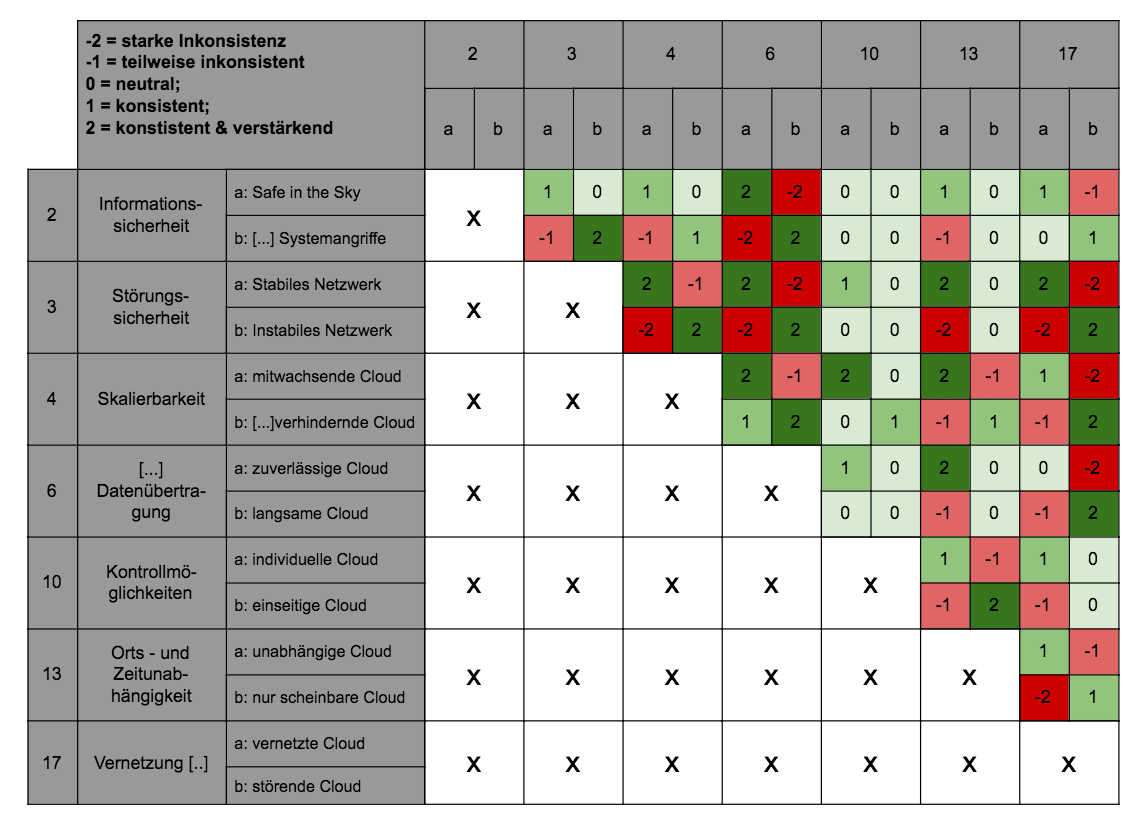
\includegraphics[width=\linewidth]{images/konsistenzanalyse}
	\caption[Caption for parameters]{Konsistenzanalyse}
	\label{fig:konsistenzanalyse}
\end{figure}

Für die Konsistenzanalyse wurde eine Skala zwischen -2 (starke Inkonsistenz) und 2 (konsistent und verstärkend) gewählt. Faktorenausprägungen, die eine starke Inkonsistenz aufweisen, können nicht zusammen in einem Szenario aufgeboten werden \cite{spath}. Andersrum können aus verstärkenden Ausprägungen Cluster gebildet werden, woraus sich Szenarien abbilden lassen.

Aus der Analyse der Schlüsselfaktoren auf Widerspruchsfreiheit lässt sich sehr gut erkennen, dass sich die jeweiligen Best-Case Ausprägungen zumeist verstärken. Besonders lässt sich ein positives Cluster aus den Ausprägungen \textit{Stabiles Netzwerk} (3a), \textit{mitwachsende Cloud} (4a), \textit{zuverlässige Cloud} (6a) und \textit{unabhängige Cloud} zusammenfassen. Andere positive Ausprägungen lassen sich zudem hinzuaddieren, sodass sie weiterhin verstärkend wirken. Im Gegensatz dazu verstärken sich die negativen Ausprägungen der Schlüsselfaktoren, wodurch sich ein entsprechendes negatives Cluster bilden lässt.

Aus dieser Betrachtung lässt sich erschließen, dass sich die Vorteile des Cloud Computing generell verstärkend aufeinander auswirken. Ebenso unterstützen sich die Risiken gegenseitig in ihrer Ausprägung. Diese Erkenntnis kann nun zur Hilfe gezogen zu werden, um drei mögliche Zukunftsszenarien für das Cloud Computing im Bildungsbreich zu erstellen.

\subsection{Szenario 1 - Mobiles Lernen auf dem Vormarsch}
\todo[inline]{Auf Cloud Modelle Abschnitt 1 zurückgreifen!}
\subsection{Szenario 2 - Blended Learning (Hybrid)}

\subsection{Szenario 3 - Zu hohe Risiken}

